\subsection*{Desastre del transbordador espacial Challenger: un análisis estadístico del accidente del Challenger}

\begin{center}  
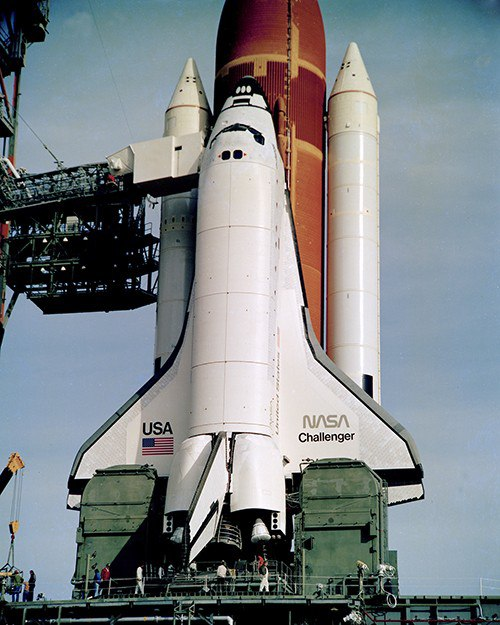
\includegraphics[width=8cm, height=10cm]{figures/challenger.jpg}
\end{center}

En la mañana del 28 de enero de 1986 en Cabo Cañaveral, el transbordador
espacial de la NASA, Challenger estaba sentado en la plataforma de despegue a
punto de despegar. Muchos vieron el evento transmitido con optimismo, mientras
aumentaba la preocupación entre los ingenieros de Thiokol (fabricante) de la
nave espacial debido a las temperaturas significativamente bajas antes del
despegue, lo que puede causar un problema con el transbordador que contiene sus
gases calientes.

La NASA ignoró estas advertencias y decidió continuar con el lanzamiento
programado. Desafortunadamente, las sospechas de los ingenieros resultaron ser
correctas; 73 segundos de vuelo. El transbordador explotó por completo. Además,
esto condujo a la muerte de los siete astronautas.

Debería haber sido un momento histórico. Pero resultó ser uno de los peores
desastres de transbordadores espaciales jamás observados. Se realizaron
investigaciones explorando las causas de la explosión del tanque de combustible
del barco. Lo que finalmente se remonta a las juntas tóricas que evitaban la
fuga de gas caliente.

Ha habido muchas acusaciones y argumentos sobre quién tiene la culpa, pero una
comprensión profunda del desastre requiere un análisis estadístico de los datos
disponibles de las juntas tóricas que contienen información sobre la temperatura
y las tasas de éxito/fallo.

Analizar las fallas de las juntas tóricas requiere una comprensión de la
estructura subyacente de Challenger. Los propulsores de cohetes del
transbordador tenían cuatro segmentos. En primer lugar, lleno de combustible. En
segundo lugar, oxidante. Y la NASA los ensambló y selló con juntas tóricas, un
componente crítico que evitó la fuga de gas caliente durante el lanzamiento.


Sin embargo, la capacidad de respuesta de los sellos no se probó en temperaturas
frías.


El día del lanzamiento, la temperatura era de 31 grados Fahrenheit,
significativamente más baja que las temperaturas en las que se probaron las
juntas tóricas. Después del despegue, una de las juntas tóricas se rompió, lo
que provocó que el gas caliente calentara el oxígeno líquido y el hidrógeno
dentro de los tanques. finalmente rompiendo los propulsores y destrozando el
transbordador 1 . Entonces, ¿por qué se tomó la decisión de continuar con el
lanzamiento, a pesar de las advertencias de los ingenieros?


Antes del lanzamiento del Challenger, nadie había analizado la asociación entre
la temperatura y la capacidad de respuesta de las juntas tóricas. La NASA
decidió arriesgarse al lanzar el transbordador, sin conocer la verdadera
probabilidad estadística de fallas en las juntas tóricas a 31 grados.

Las preocupaciones de los ingenieros se basaban en sospechas y análisis
incompletos. Los ingenieros solo observaron los datos de las juntas tóricas de
baja temperatura que incluían 4 fallas. Al ignorar los datos sobre vuelos a
temperaturas más altas, la probabilidad de falla calculada fue menor de lo que
debería haber sido 2. Este análisis no solo es incorrecto sino también
peligroso y condujo al desastre.

Se deben tener en cuenta los datos de todos los vuelos que se registraron. Ha
habido muchas fallas de juntas tóricas tanto a altas como a bajas temperaturas,
pero no se ha medido la fuerza de la asociación entre estas dos variables. Los
ingenieros no pueden simplemente ignorar los vuelos con temperaturas más
altas.

Se requiere un análisis estadístico profundo de la eficiencia de las juntas
tóricas a varias temperaturas para comprender realmente la falla del Challenger.
Las intuiciones y los análisis sesgados, especialmente por parte de la
administración de la NASA, no son suficientes para determinar la probabilidad de
falla de las juntas tóricas.

A continuación se muestra una muestra de los datos de fallas de las juntas
tóricas:

\begin{center}  
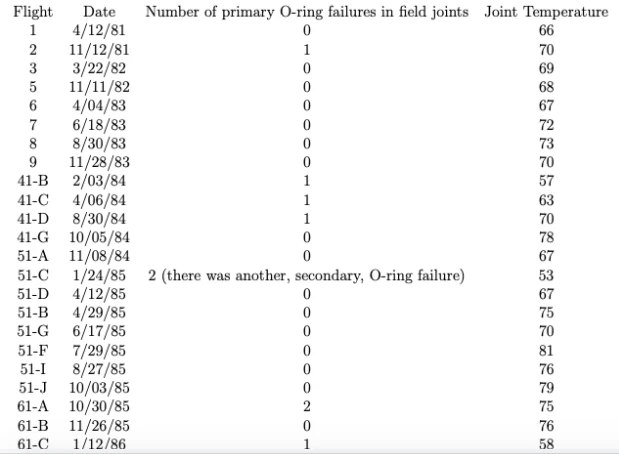
\includegraphics{figures/challenger_data.jpg}
\end{center}

Muestra de datos de juntas tóricas 3.

Se puede ejecutar una prueba de permutación para evaluar la importancia
estadística de la diferencia entre la tasa de falla de la junta tórica a bajas
temperaturas y la tasa de falla a altas temperaturas. Esto puede determinar si
las juntas tóricas de temperatura más baja tienden a experimentar más fallas que
las juntas tóricas de temperatura alta, o si la distribución de fallas es la
misma entre las dos. Las hipótesis de esta prueba estadística son las
siguientes:


\begin{center}  
$H_o: Falla_{bajaTemperatura} - Falla_{altaTemperatura} = 0$
\end{center}


La verdadera diferencia media entre la tasa de falla de la junta tórica a baja y
alta temperatura es 0. Las diferencias observadas se deben al azar.


\begin{center}  
$H_o: Falla_{bajaTemperatura} - Falla_{altaTemperatura} > 0$
\end{center}


La verdadera diferencia media entre la tasa de falla de la junta tórica a baja y
alta temperatura es mayor que 0. Las diferencias observadas no se deben al azar,
sino a una asociación entre la temperatura y la tasa de falla.

La permutación se ejecuta agrupando cada punto de datos en dos grupos. Alta y
baja temperatura. Mirando la distribución de temperatura. Las observaciones de
juntas tóricas se pueden dividir en menos de 65 grados (baja temperatura). Y por
encima de 65 grados (alta temperatura).

La diferencia media observada de fallos entre juntas tóricas de baja y alta
temperatura es de 1,3; la columna de temperatura se permuta (baraja). Y la
diferencia de falla media simulada la calculamos nuevamente entre los dos grupos
de juntas tóricas. La ejecución de 10 000 simulaciones de esta prueba de
permutación produce 10 000 estadísticas de prueba simuladas. A partir de esto,
podemos calcular el valor $p$ para evaluar la hipótesis nula:


\begin{center}  
\begin{align*} 
\frac{sum(diferencias\;simuladas> diferencia\;observada)}{total\; intentos}) = \frac{sum(diferencias \;simuladas>1.3)}{1000}= \\
=0.012
\end{align*}
\end{center}



Solo el $1,2 \%$ de las diferencias medias de fallas simuladas son mayores que
la diferencia media de fallas observada. Un valor p de 0.012 es estadísticamente
significativo para rechazar la hipótesis nula que establece que las tasas de
falla de las juntas tóricas en temperaturas bajas y altas provienen de la misma
distribución.

La diferencia observada es mucho mayor que las diferencias en los datos de las
juntas tóricas barajadas. Esto sugiere que la tasa de fallas entre las juntas
tóricas de baja y alta temperatura no tiene la misma distribución. \\Los datos
muestran evidencia que respalda la hipótesis alternativa que establece que las
juntas tóricas de baja temperatura tienen una mayor tasa media de fallas que las
juntas tóricas de alta temperatura.

Definitivamente parece haber una diferencia entre las juntas tóricas probadas a
bajas temperaturas. Y las juntas tóricas se probaron a altas temperaturas, pero
es útil examinar el modelo subyacente de los datos.

Es importante estimar la probabilidad de falla de la junta tórica a una
temperatura determinada. Esto se puede hacer ajustando un modelo de regresión
logística a los datos anteriores. Con temperatura como entrada y un valor
binario (1: al menos una falla, 0: ninguna falla) como salida. Ajustamos una
regresión logística con los siguientes parámetros:


\begin{center}  
$P(Falla)= \frac{1}{1+exp^{-(\beta_0+\beta_1*temperatura)}}$
\end{center}

Cuando:

\begin{center}  
$\beta_1$
\end{center}

es el coeficiente de temperatura que mide la asociación y


\begin{center}  
$\beta_0$
\end{center}


es el sesgo.

Además, probamos la fuerza de la asociación calculando un valor z con respecto a
las siguientes hipótesis:



\begin{center}  
$H_0 : \beta_1 = 0$
\end{center}


El verdadero coeficiente de temperatura para el modelo es 0, lo que indica que
no hay relación entre la temperatura y la falla de la junta tórica.


\begin{center}  
$H_0 : \beta_1 \not {0}$
\end{center}

El verdadero coeficiente de temperatura para el modelo no es 0, lo que indica
alguna relación entre la temperatura y la falla de la junta tórica.\\

Ajustar los datos a una regresión logística genera un modelo con los siguientes
pesos:

\begin{center}  
$P(Falla)= \frac{1}{1+exp^{-(10.88+0.17*temperatura)}}$
\end{center}


Una gráfica a continuación visualiza la distribución de fallas y el ajuste del modelo:


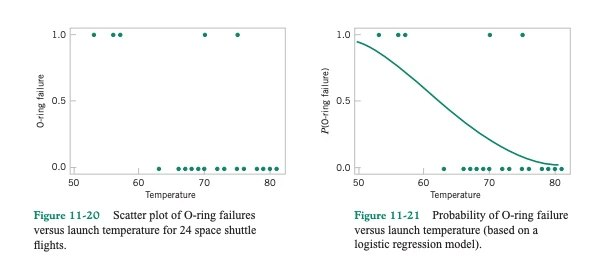
\includegraphics[width=15cm, height=10cm]{figures/challenger_plots.jpg}

Gráfica de regresión logística de datos de juntas tóricas 

Como se observa en la gráfica, una temperatura de 31 grados parece
increíblemente probable que tenga al menos una falla. El modelo genera un valor
de 0,996, lo que indica un $99,6 \%$ de probabilidad de falla dados los datos
observados de lanzamientos de transbordadores anteriores.

Esto está lejos de ser una decisión cerrada y ciertamente no es una apuesta
arriesgada cuando hay siete compañeros de tripulación a bordo.

Además, la fuerza de la asociación entre estas dos variables. Analizamos con el
estadístico z generado en el peso del modelo del coeficiente de temperatura. El
valor $p$ calculado de la hipótesis nula:


\begin{center}  
$H_0 : \beta_1 = 0$
\end{center}


resulta ser 0,04, que es estadísticamente significativo cuando se utiliza un
umbral de 0,05. Debido al bajo valor de p, rechazamos la hipótesis nula que
establece que el coeficiente de temperatura es 0. Existe una fuerte evidencia en
los datos que respalda la hipótesis alternativa:

\begin{center}  
$H_0 : \beta_1 > 0$
\end{center}


lo que sugiere que el coeficiente es mayor que 0 y que, de hecho, existe una
asociación entre la temperatura y la falla de la junta tórica. Por lo tanto,
existe una fuerte evidencia de que las bajas temperaturas pueden provocar fallas
en las juntas tóricas. Además, los ingenieros deberían haber presentado un
análisis de regresión logística como evidencia para retrasar el lanzamiento del
Challenger.\\

Hay muchas explicaciones posibles de por qué los funcionarios de la NASA
decidieron ignorar todas las advertencias de los ingenieros de Thiokol y
continuar con el lanzamiento. Algunos dicen que se debió al simple hecho de que
la NASA quería demostrar que otros estaban equivocados y mantener su ambicioso
programa de lanzamiento.\\

Otros argumentan que se debió a razones burocráticas. La Casa Blanca presionó a
la NASA para realizar el lanzamiento. Entonces Reagan podría mencionarlo en su
discurso sobre el estado de la unión. Además, la dirección se produjo el mismo
día. No importa la razón, la NASA no debería haber hecho una apuesta tan grande
y debería haber retrasado el lanzamiento para otro día.\\
El análisis de los datos retrata claramente los riesgos, pero nadie había hecho
una investigación exhaustiva de antemano. Como resultado del desastre, el
Congreso cerró el programa de transbordadores espaciales durante años. Hasta que
la NASA abordó sus problemas internos.\\

La NASA hizo una extensa investigación sobre sus propios fracasos. Y la NASA
implementó cambios significativos para abordar las incompetencias existentes.
Además, la NASA publicó informes de investigación que describen la incapacidad
de la junta tórica para mantener su elasticidad después de la exposición a bajas
temperaturas.\\

La Casa Blanca formó un comité presidencial para investigar asuntos internos en
la NASA. Y supervisar la reestructuración de la planificación y gestión de
misiones. La NASA remodeló una parte significativa del diseño actual del
transbordador para reducir los riesgos de puntos de falla.\\

Capacitación de gestión fuertemente aplicada por la NASA. Esto cambió la
dinámica de la cultura laboral. Los funcionarios y los ingenieros fueron todos
responsables de abordar todas las inquietudes que surgieron durante el proceso
de lanzamiento 5 . La NASA tardó dos años en reparar los daños, reestructurar y
reabrir.\\
Este desastre se convirtió en la base para que la NASA mejorara su toma de
decisiones y la coordinación entre ingenieros y administradores. Después de
cambiar las operaciones internas y establecer nuevos estándares éticos y de
producción, la NASA continuó con su programa de transbordadores espaciales con
misiones mejor administradas. Discovery fue la primera misión después de la
reapertura y transcurrió sin problemas. Esto se convirtió en el advenimiento de
una serie de misiones exitosas aprendiendo de los errores cometidos en
Challenger.\\

El desastre del Challenger muestra por qué los científicos e ingenieros
necesitan comprender las técnicas estadísticas. Los análisis básicos descritos
brindan una sólida evidencia cuantitativa de que el transbordador no debería
haberse lanzado debido a la probabilidad significativamente alta de falla de la
junta tórica, un componente crítico de la nave espacial.\\

La NASA ahora ha hecho del análisis estadístico y de riesgo de cada componente
del transbordador una prioridad antes del lanzamiento. Es probable que este
estándar prevenga muchos desastres futuros y promueva la expansión del programa
de exploración espacial de los Estados Unidos.\\

